\documentclass{beamer}
\usepackage[utf8]{inputenc}
\usepackage{booktabs}
\usepackage{graphicx}
\usepackage{amsmath}
\usepackage{amssymb}

\usetheme{Madrid}
\usecolortheme{default}

\title{Wireless Channel Fingerprinting and Charting}
\subtitle{Ray-Tracing Dataset Generation, Localization, and Dimensionality Reduction}
\author{Jari Karppinen \\ Hannu Flinck \\ Tommi Ylämurto}
\institute{Machine Learning for Wireless Communications \\ Aalto University}
\date{\today}

\begin{document}

\begin{frame}
\titlepage
\end{frame}

\begin{frame}
\frametitle{Table of Contents}
\tableofcontents
\end{frame}

% =============================================================================
% SECTION 1: INTRODUCTION AND BACKGROUND
% =============================================================================
\section{Introduction and Background}

\begin{frame}
\frametitle{Urban Radio Propagation}
\begin{columns}
\column{0.5\textwidth}
\begin{itemize}
  \item Urban environments exhibit rich multipath propagation
  \item Dominant mechanisms:
  \begin{itemize}
    \item Specular reflection from building facades
    \item Diffraction at building edges
    \item Transmission through exterior walls
  \end{itemize}
  \item Key channel descriptors:
  \begin{itemize}
    \item RMS delay spread
    \item Angular spread of arrival/departure
    \item Aggregate path loss
  \end{itemize}
\end{itemize}

\column{0.5\textwidth}
\centering
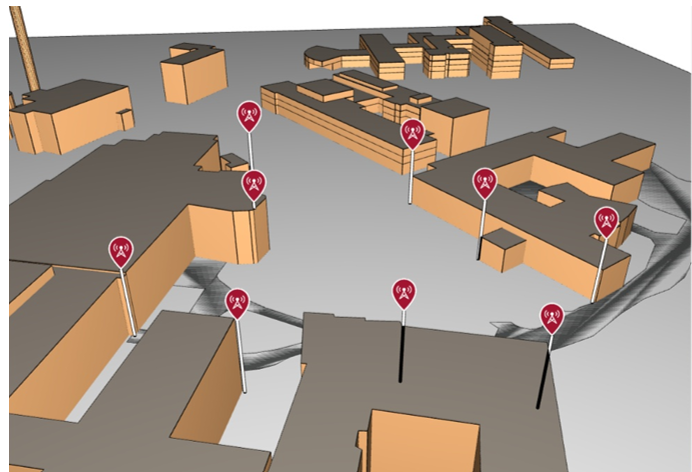
\includegraphics[width=0.95\columnwidth]{pictures/tommi/Simulated_environment.png}
\end{columns}
\end{frame}

\begin{frame}
\frametitle{Ray-Tracing for Channel Modelling}
\begin{itemize}
  \item Deterministic propagation modelling technique
  \item Simulates geometric and electromagnetic interactions of rays with surfaces
  \item Advantages over stochastic models:
  \begin{itemize}
    \item Directly exploits site-specific scene information
    \item Produces physically realistic channel characteristics
    \item Enables site-dependent analysis
  \end{itemize}
\end{itemize}

\vspace{0.5cm}
\textbf{Dataset Generation:}
\begin{itemize}
  \item MATLAB's Ray Tracing Toolbox
  \item OpenStreetMap-derived 3-D model
  \item Configurable parameters: reflections, diffractions, frequency
\end{itemize}
\end{frame}

% =============================================================================
% SECTION 2: MEASUREMENT SCENARIO AND DATASET
% =============================================================================
\section{Otaniemi Scenario and Dataset}

\begin{frame}
\frametitle{Otaniemi Campus Setup}
\begin{columns}
\column{0.5\textwidth}
\textbf{Scene Geometry:}
\begin{itemize}
  \item Location: Espoo, Finland
  \item Area: $132 \times 147$ meters
  \item Building model from OpenStreetMap
  \item Material properties: concrete (walls), metal (roofs), loam (ground)
\end{itemize}

\vspace{0.3cm}
\textbf{Radio Configuration:}
\begin{itemize}
  \item Frequency: 3.6 GHz (5G NR Band n78)
  \item 9 rooftop base stations
  \item 16-element $4 \times 4$ antenna arrays per BS
  \item UE grid: $2.5\,\text{m}$ spacing
  \item Total UE positions: 3,069
\end{itemize}

\column{0.5\textwidth}
\centering
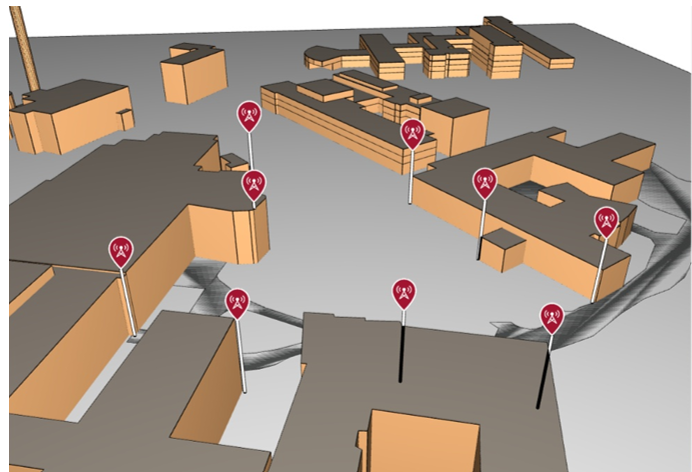
\includegraphics[width=0.95\columnwidth]{pictures/tommi/Simulated_environment.png}
\end{columns}
\end{frame}

\begin{frame}
\frametitle{MATLAB Ray-Tracing Dataset}
\begin{columns}
\column{0.5\textwidth}
\textbf{Feature Extraction:}
\begin{itemize}
  \item Ray tracing parameters:
  \begin{itemize}
    \item Max reflections: 4
    \item Max diffractions: 2
    \item Retained paths per link: 40 strongest
  \end{itemize}
  \item Two feature branches:
  \begin{itemize}
    \item Antenna-domain features (AoA, covariance)
    \item Frequency-domain features (CSI)
  \end{itemize}
\end{itemize}

\vspace{0.3cm}
\textbf{Final Feature Set (63 dimensions):}
\begin{itemize}
  \item Angle-of-Arrival (AoA)
  \item Received Signal Strength (RSS)
  \item Path Delay
  \item LOS Indicator
\end{itemize}

\column{0.5\textwidth}
\centering
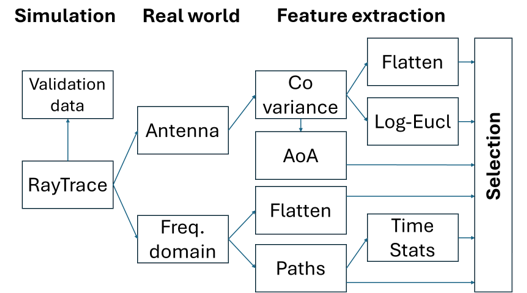
\includegraphics[width=0.95\columnwidth]{pictures/tommi/Workflow_for_creating_the_features.png}
\end{columns}
\end{frame}

% =============================================================================
% SECTION 3: FINGERPRINT LOCALIZATION
% =============================================================================
\section{Fingerprint Localization}

\begin{frame}
\frametitle{Localization Methods}
\begin{itemize}
  \item \textbf{Non-parametric:} wKNN (IDW) with $k=3$ and Minkowski $p=3$
  \item \textbf{Neural Regressors:}
  \begin{itemize}
    \item MLP: fully-connected, 4 hidden layers
    \item CNN: 1-D/2-D convolutional with cross-BS convolutions
  \end{itemize}
  \item \textbf{Ensemble:} Average of 5 independently-initialised MLPs
  \item \textbf{Classification:} MLP mapping to $2.5\,\text{m}$ grid cells (fails due to sparsity)
\end{itemize}

\vspace{0.5cm}
\textbf{Evaluation Metrics:}
\begin{itemize}
  \item Mean Absolute Error (MAE)
  \item Root Mean Square Error (RMSE)
  \item Error percentiles (P90, P95)
\end{itemize}
\end{frame}

\begin{frame}
\frametitle{Localization Results}
\begin{table}[h]
\small
\centering
\caption{MATLAB Dataset Performance ($N_{\text{test}} = 921$, $D_f = 63$)}
\begin{tabular}{lrrrrr}
\toprule
Method & MAE (m) & RMSE (m) & Median (m) & P90 (m) & P95 (m) \\
\midrule
wKNN (IDW) & 18.24 & 27.25 & 10.14 & 46.08 & 65.34 \\
wKNN C2F & 18.18 & 30.05 & 7.16 & 57.23 & 75.35 \\
NN Regression & 19.79 & 29.03 & 11.06 & 54.70 & 71.93 \\
CNN Regression & 20.40 & 28.94 & 12.51 & 54.06 & 71.37 \\
Ensemble (5 MLPs) & 18.38 & 27.85 & 9.64 & 55.09 & 68.40 \\
\bottomrule
\end{tabular}
\end{table}

\begin{columns}
\column{0.5\textwidth}
\centering
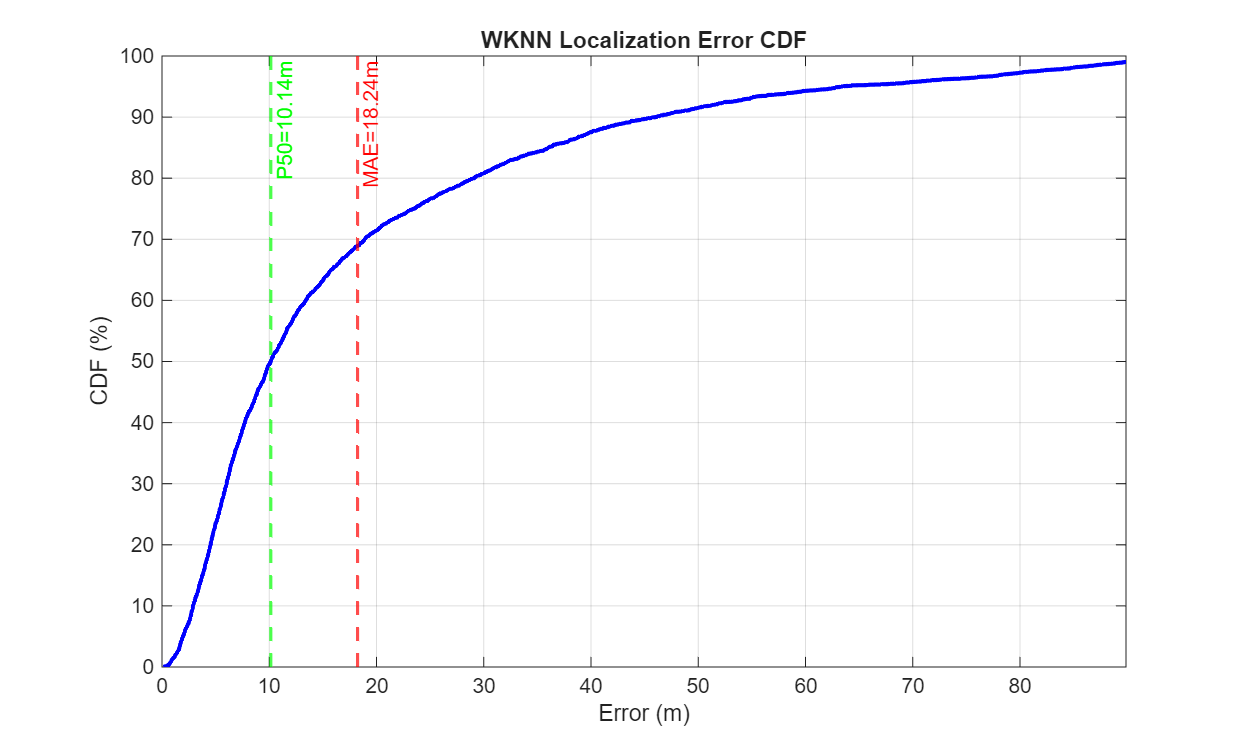
\includegraphics[width=0.95\columnwidth]{pictures/03_localization/wknn_cdf_1.png}

\column{0.5\textwidth}
\centering
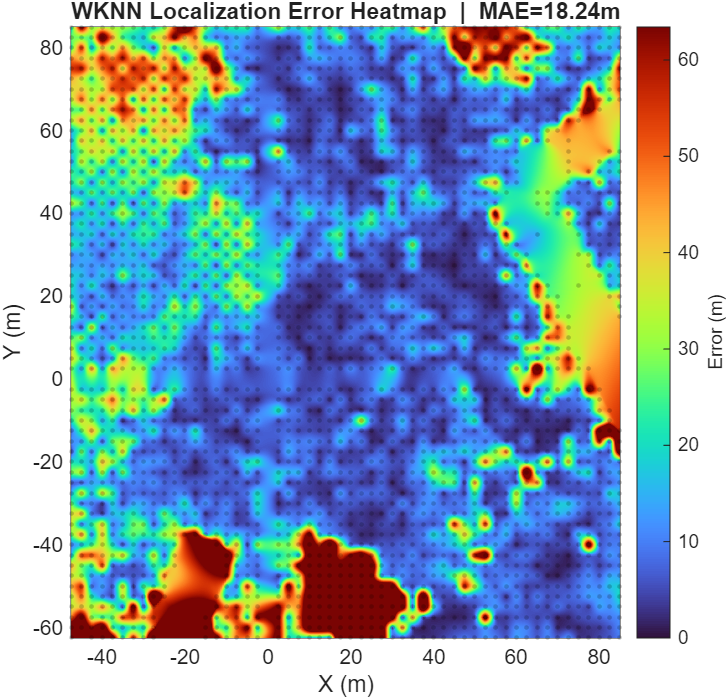
\includegraphics[width=0.95\columnwidth]{pictures/03_localization/wknn_error_heatmap.png}
\end{columns}
\end{frame}

\begin{frame}
\frametitle{Key Findings: Localization}
\begin{itemize}
  \item \textbf{wKNN Coarse-to-Fine (C2F)} achieves best median error: 7.16 m
  \item \textbf{Ensemble methods} provide robust performance with stable tails
  \item \textbf{Classification fails} due to sparse grid (3,069 cells vs. $\sim$2,148 training samples)
  \item \textbf{Dominant error source:} Spatial ambiguity in NLOS shadow regions behind large facades
  \item \textbf{Fingerprinting robust} across different ray-tracing implementations (MATLAB validation confirms)
\end{itemize}
\end{frame}

% =============================================================================
% SECTION 4: CHANNEL CHARTING
% =============================================================================
\section{Channel Charting}

\begin{frame}
\frametitle{Channel Charting Methods}
\textbf{Goal:} Produce low-dimensional representation preserving neighbourhood structure without position labels

\vspace{0.3cm}
\begin{itemize}
  \item \textbf{PCA:} Linear principal-component projection (baseline)
  \item \textbf{t-SNE:} Non-linear stochastic neighbour embedding
  \begin{itemize}
    \item Perplexity sweep: $\{5, 15, 30, 50\}$
    \item Best: perplexity = 30
  \end{itemize}
  \item \textbf{Autoencoder:} Symmetric encoder/decoder with 2-D bottleneck
  \item \textbf{UMAP:} Uniform manifold approximation and projection
  \begin{itemize}
    \item Neighbourhood size sweep: $\{5, 10, 20, 30\}$
    \item Best: $n_{\text{neighbors}} = 5$
  \end{itemize}
\end{itemize}

\vspace{0.3cm}
\textbf{Preprocessing:} 50 PCA components for t-SNE and UMAP (noise reduction)
\end{frame}

\begin{frame}
\frametitle{Channel Charting Evaluation Metrics}
\begin{itemize}
  \item \textbf{Trustworthiness (TW, $\uparrow$):} Penalises false neighbours (close in chart, far in RF space)
  \item \textbf{Continuity (CT, $\uparrow$):} Penalises tears (close in RF space, far in chart)
  \item \textbf{Kolmogorov--Smirnov Distance (KS, $\downarrow$):} Compares pairwise-distance distributions
  \begin{itemize}
    \item $\text{KS} \to 0$ = globally scale-preserving chart
  \end{itemize}
  \item \textbf{NNLE ($\downarrow$, m):} Nearest-neighbour localization error
  \begin{itemize}
    \item Predicts UE position from chart's nearest neighbour
    \item Ties chart quality to downstream task
  \end{itemize}
\end{itemize}

\vspace{0.3cm}
\textbf{Ideal Chart:} $\text{TW} \approx \text{CT} \approx 1$, $\text{KS} \approx 0$, $\text{NNLE}$ $\sim$ grid spacing
\end{frame}

\begin{frame}[fragile]
\frametitle{Channel Charting Results}

\vspace{-0.2cm}
\begin{table}[h]
\tiny
\centering
\begin{tabular}{lcccc}
\toprule
Method & TW $\uparrow$ & CT $\uparrow$ & KS $\downarrow$ & NNLE (m) $\downarrow$ \\
\midrule
PCA & 0.706 & 0.932 & 0.514 & n/a \\
\textbf{t-SNE (30)} & \textbf{0.918} & \textbf{0.958} & \textbf{0.451} & \textbf{8.35} \\
Autoencoder & 0.850 & 0.920 & 0.771 & 22.00 \\
UMAP ($n=5$) & 0.896 & 0.914 & 0.861 & 10.92 \\
\bottomrule
\end{tabular}
\end{table}

\vspace{-0.3cm}
\begin{columns}[T]
\column{0.5\textwidth}
\centering
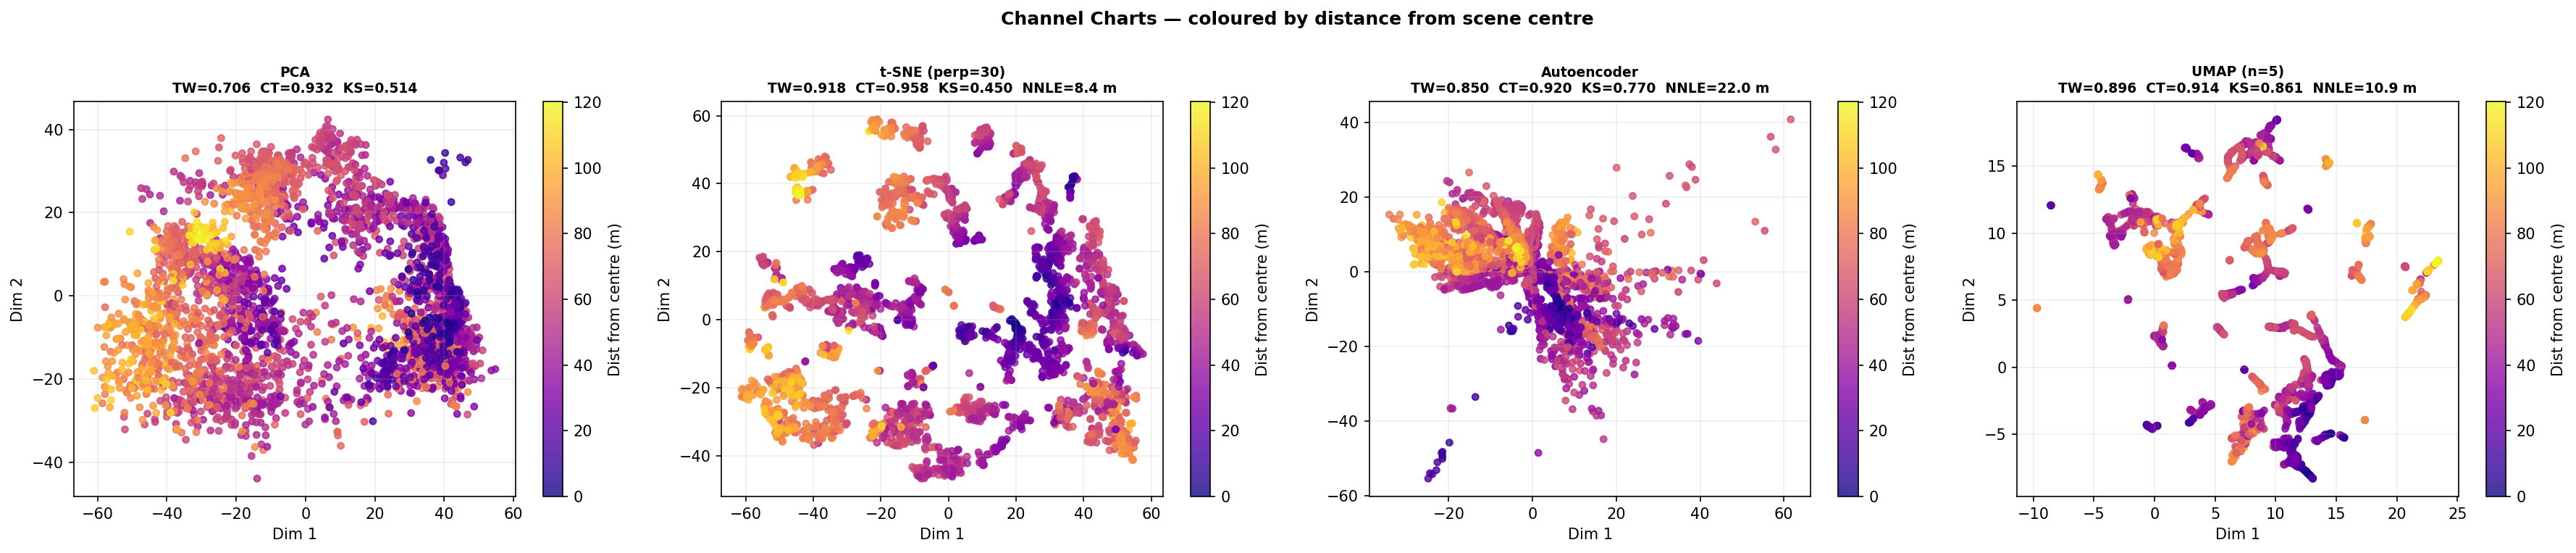
\includegraphics[width=1.0\columnwidth]{pictures/04_channel_charting/channel_charts_comparison.png}

\column{0.5\textwidth}
\centering
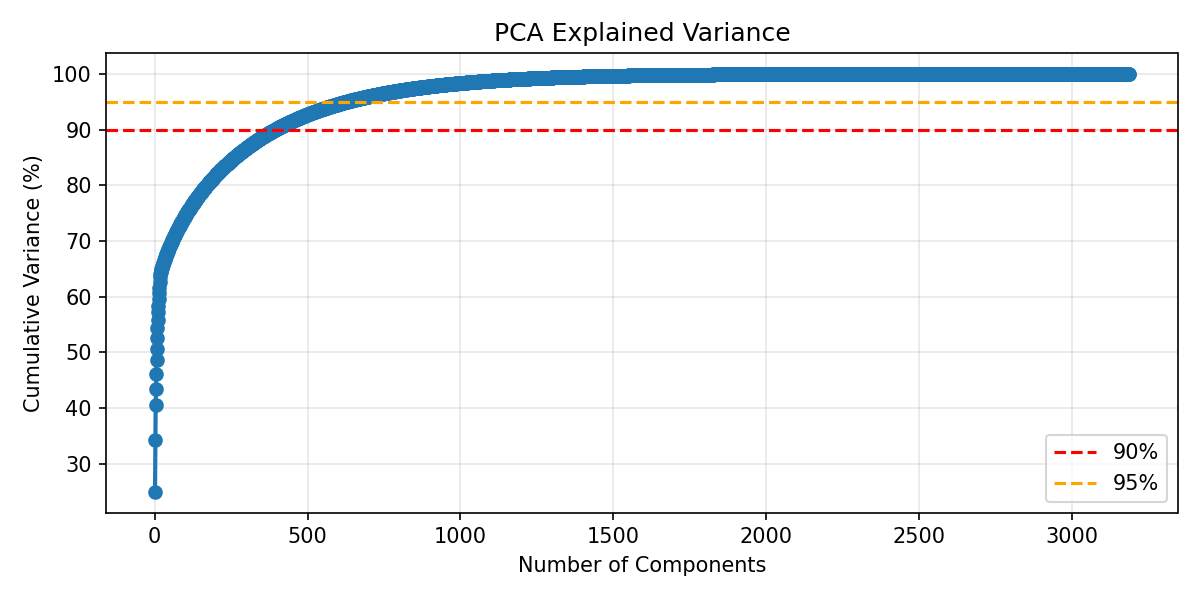
\includegraphics[width=1.0\columnwidth]{pictures/04_channel_charting/pca_explained_variance.png}
\end{columns}
\end{frame}

\begin{frame}
\frametitle{Key Findings: Channel Charting}
\begin{itemize}
  \item \textbf{t-SNE dominates} across all metrics: TW=0.918, CT=0.958, KS=0.451
  \item \textbf{NNLE = 8.35 m} comparable to best supervised regressor without UE labels
  \item \textbf{UMAP trades} neighbourhood TW against global KS
  \item \textbf{Autoencoder limited} by MSE reconstruction objective (no metric preservation)
  \item \textbf{PCA baseline:} Preserves global structure but poorly preserves local topology
  \item \textbf{Cross-validation:} MATLAB dataset shows t-SNE robustness (TW=0.975, CT=0.945)
\end{itemize}
\end{frame}

% =============================================================================
% SECTION 5: CONCLUSIONS AND FUTURE WORK
% =============================================================================
\section{Conclusions and Future Work}

\begin{frame}
\frametitle{Summary of Results}
\begin{itemize}
  \item \textbf{Dataset:} MATLAB ray-tracing on Otaniemi campus with independent validation
  \item \textbf{Localization:} wKNN C2F achieves 7.16 m median error; ensemble methods robust
  \item \textbf{Channel Charting:} t-SNE produces geometrically faithful maps (TW=0.918, NNLE=8.35 m)
  \item \textbf{Insights:}
  \begin{itemize}
    \item Fingerprinting robust across ray-tracing implementations
    \item Regression superior to classification for dense spatial grids
    \item Unsupervised charting competitive with supervised localization
  \end{itemize}
  \item \textbf{Limitations:}
  \begin{itemize}
    \item NLOS shadow regions cause ambiguity and inflated error tails
    \item Limited training samples constrain deep learning approaches
  \end{itemize}
\end{itemize}
\end{frame}

\begin{frame}
\frametitle{Future Work}
\begin{itemize}
  \item \textbf{Enhanced Features:} Incorporate per-path AoA/AoD angles from ray-tracing output
  \item \textbf{Metric-Preserving Loss:} Replace MSE autoencoder with Siamese/triplet loss
  \item \textbf{Larger Scene:} Extend to full 77-building Otaniemi model (GPU acceleration needed)
  \item \textbf{Semi-Supervised Charting:} Use small subset of labelled anchors to regularise latent space
  \item \textbf{Practical Demonstration:} Beam-management or handover policy based on learned radio-space embedding
\end{itemize}
\end{frame}

\end{document}
